\subsection{Вертикальное распределение температуры в океане. Солёность океана.}
Стандартный температурный профиль в океане включает в себя (см. рис. \ref{fig:T(h)}):
\begin{enumerate}
\item Холодную плёнку. Тонкий слой (несколько мм) у поверхности, где температура воды резко уменьшается (градиент температуры может достигать порядка нескольких тысяч град/м). Через этот слой происходит выведение тепла в атмосферу посредством молекулярного обмена.
\item Верхний квазиоднородный (перемешанный) слой (до 200 м).
\item Термоклин.
\item Глубинный слой.
\end{enumerate}

\begin{figure}[!ht]
\centering
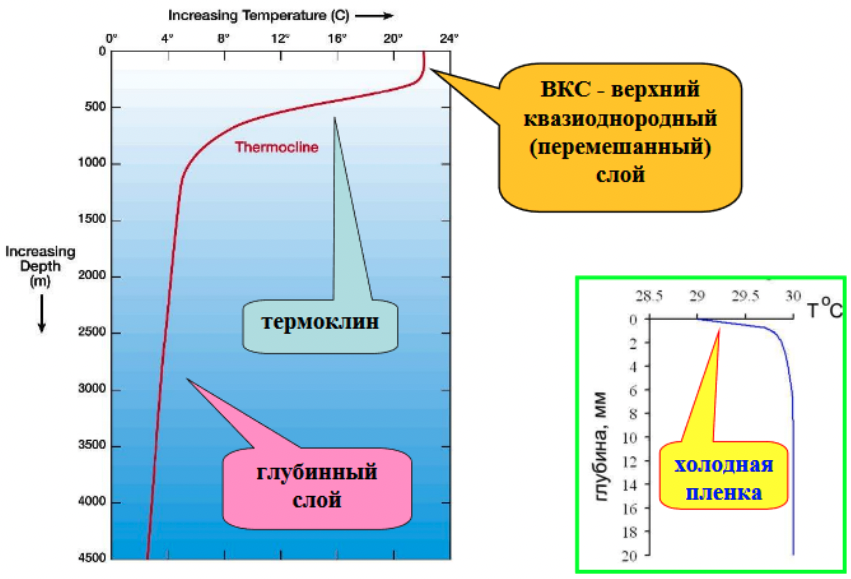
\includegraphics[width=0.5\textwidth]{images/T(h).png}
\caption{Типичный вертикальный профиль температуры в океане \cite{Nosov2019-3}.}\label{fig:T(h)}
\end{figure}

Солёность воды определяется формулой:
\begin{equation}
s=\frac{m_\text{примеси}}{m_\text{примеси}+m_\text{чистой воды}}
\end{equation}

Типичное значение солёности: в океане -- 35 \textperthousand, в реках -- 0.5 \textperthousand.
